\chapter{Lec 22 - Natural Language Processing II}

\section{Chain rule for \textit{n}-grams}
The probability of a sentence $W$ (sequence of words), is given by:
\[P(w_1, ..., w_n)\]
while a language model computes the probability
\[P(w_n| w_{1:n-1})\]
Then, Chain rule can be used to calculate the joint probability of
words:
\[P(w_1, ..., w_n) = \prod_i P(w_i | w_{1:i-1})\]
For example, the probability of the sentence "Today is hot" is given by:
\[P(\text{Today is hot}) = P(\text{Today})P(\text{is}|\text{Today})P(\text{hot}|\text{Today is})\]
How to estimate these probabilities? We cannot estimate them by considering all the combinations of words in a corpus, since we will never see enough data to estimate such probabilities.\\\\
Then, as we did for $n$-grams models for characters, we can simplify by making a Markov assumption:
\[P(w_1, ..., w_n) = \prod_i P(w_i | w_{1:i-1}) = \prod_i P(w_i | w_{i-k:i-1})\]
where $k$ determines which $n$-gram we are considering ($k=1$ bigram, $k=2$ trigram, etc.). Then, we can estimate the probability of $P(w_i|w_{i-1})$ directly from the corpus as follows:
\[P(w_i|w_{i-1}) = \frac{Count(w_i, w_{i-1})}{Count(w_{i-1})}\]


\section{Text classification}
We now consider the task of \textbf{text classification}: given a text of some kind, decide which of a predefined set of classes it belongs to. We can treat spam detection as a problem in supervised learning. A training set is readily available: the positive (spam) examples are in my spam folder, the negative (ham) examples are in my inbox.\\\\
We can have two different ways to approach the classification of the text:
\begin{itemize}
    \item Use of hand-coded classification rules
    \item Use of linguistic modeling and machine learning
\end{itemize}
If the rules are carefully refined by an expert, the accuracy can be high, but building such rules is very expensive and not always possible.\\\\
In the language-modeling approach, we define one $n$-gram language model for $\textbf{P}(Message | spam)$, by training on the spam folder, and one model for $\textbf{P}(Message | ham)$ by training on the inbox. Then we can classify a new message with an application of Bayes’ rule:
\[argmax_{c \in \{spam, ham\}} P(c|message) = argmax_{c \in \{spam, ham\}} P(message|c)P(c)\]
where $P(c)$ is estimated just by counting the total number of spam and ham messages. Assume that each message is made of $n$ tokens $x_i$. Then, the Bayes' rule can be rewritten as:
\[argmax_{c \in \{spam, ham\}} P(c|message) = argmax_{c \in \{spam, ham\}} P(x_1, ..., x_n|c)P(c)\]
Estimate $P(x_1, ..., x_n|c)$ is usually unfeasible since we don't have enough data to do it. Then, we need to rely on some approximation. In particular, we can exploit conditional independence. Basically, we assume that all the tokens are conditionally independent, given $c$, i.e., $P(x_1, ..., x_n|c) = \prod_i P(x_i|c)$, which leads to the definition of Multinomial Naive Bayes Classifier:
\[c_{NB} = argmax_{c \in \{spam, ham\}} P(c)\prod_i P(x_i|c)\]

\section{Text representation}
In the machine-learning approach we represent the message as a set of feature/value
pairs and apply a classification algorithm $h$ to the feature vector $\textbf{X}$. How can we represent a message?

\subsection{Bag-of-Words}
Bag-of-Words is a way to convert text data into a numerical format that machine learning algorithms can work with. The term "bag of words" implies that the order of words is disregarded, and the focus is solely on the presence or absence of words in a document.\\\\
The idea is to think of the $n$-grams as features. This is easiest to see with a unigram model. The features are the words in the vocabulary, and the values are the number of times each word appears in the message. That makes the feature vector large and sparse. This unigram representation has been called the bag of words model.
\\\\
The notion of order of the words is lost; a unigram model gives the same probability to any permutation of a text. . Higher-order $n$-gram models maintain some local notion of word order, but the computational complexity increases with the order.\\\\
Representing words as discrete symbols has a big problem: there is no notion of similarity between any encoding vector, even if the sentences are semantically similar. We have 2 possible solutions:
\begin{itemize}
    \item "Knowledge representation way": can rely on a list of synonyms or taxonomies of words (for example WordNet) to obtain similarity.

    \item "Machine learning way": learning to code the similarity in the vectors themselves.
\end{itemize}

\subsection{Word Embedding - Word2Vec}
(Neural) \textbf{Word embedding} belongs to the text pre-processing phase. The goal is to transform a text (set of words) into a vector of numbers such that similar words produce similar vectors. The word2vec technique is based on a feed-forward, fully connected architecture. It is similar to an autoencoder, but rather than performing input reconstruction, word2vec trains words according to other words that are neighbors in the input corpus (called \textbf{context}).\newline\newline
Word2vec aims at computing a \textbf{vector} representation of words able to capture semantic and syntactic word similarity.\newline\newline
By using this concept of context, word2vec can learn word embedding in two different ways:
\begin{itemize}
    \item \textbf{CBOW} (Continuous Bag of Words) in which the neural network uses the context to predict a target word.

    \item \textbf{Skip-gram} in which it uses the target word to predict a target context.
\end{itemize}
\begin{center}
    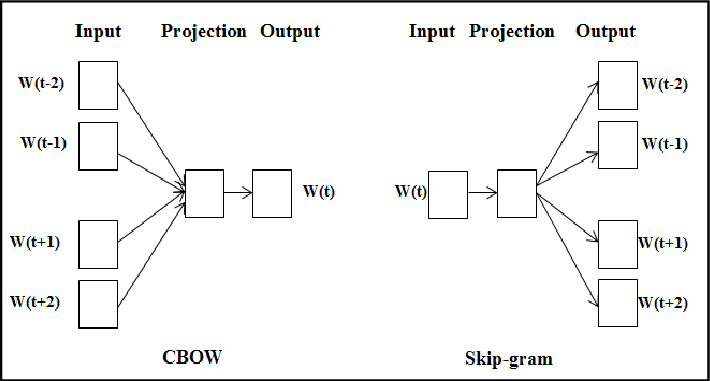
\includegraphics[scale = 0.3]{images/word2vec.png}
\end{center}

\subsubsection{Word2Vec Skip-gram model}
The input of the model is the one-hot encoding of the word according to a vocabulary.
The output is a distribution over the words of being in the context of the target word. The formal method is defined as follows:
\[\textbf{h} = \textbf{W}^{T}\textbf{x}\]
\[\textbf{u} = \textbf{W}^{'T}\textbf{h} = \textbf{W}^{'T}\textbf{W}^{T}\textbf{x}\]
\[\textbf{y} = \sigma(\textbf{u})\]
where $\sigma(\cdot)$ is the \textbf{softmax} function.\newline\newline
The goal of skip-gram model is to maximize the \textbf{average log probability}.
\begin{center}
    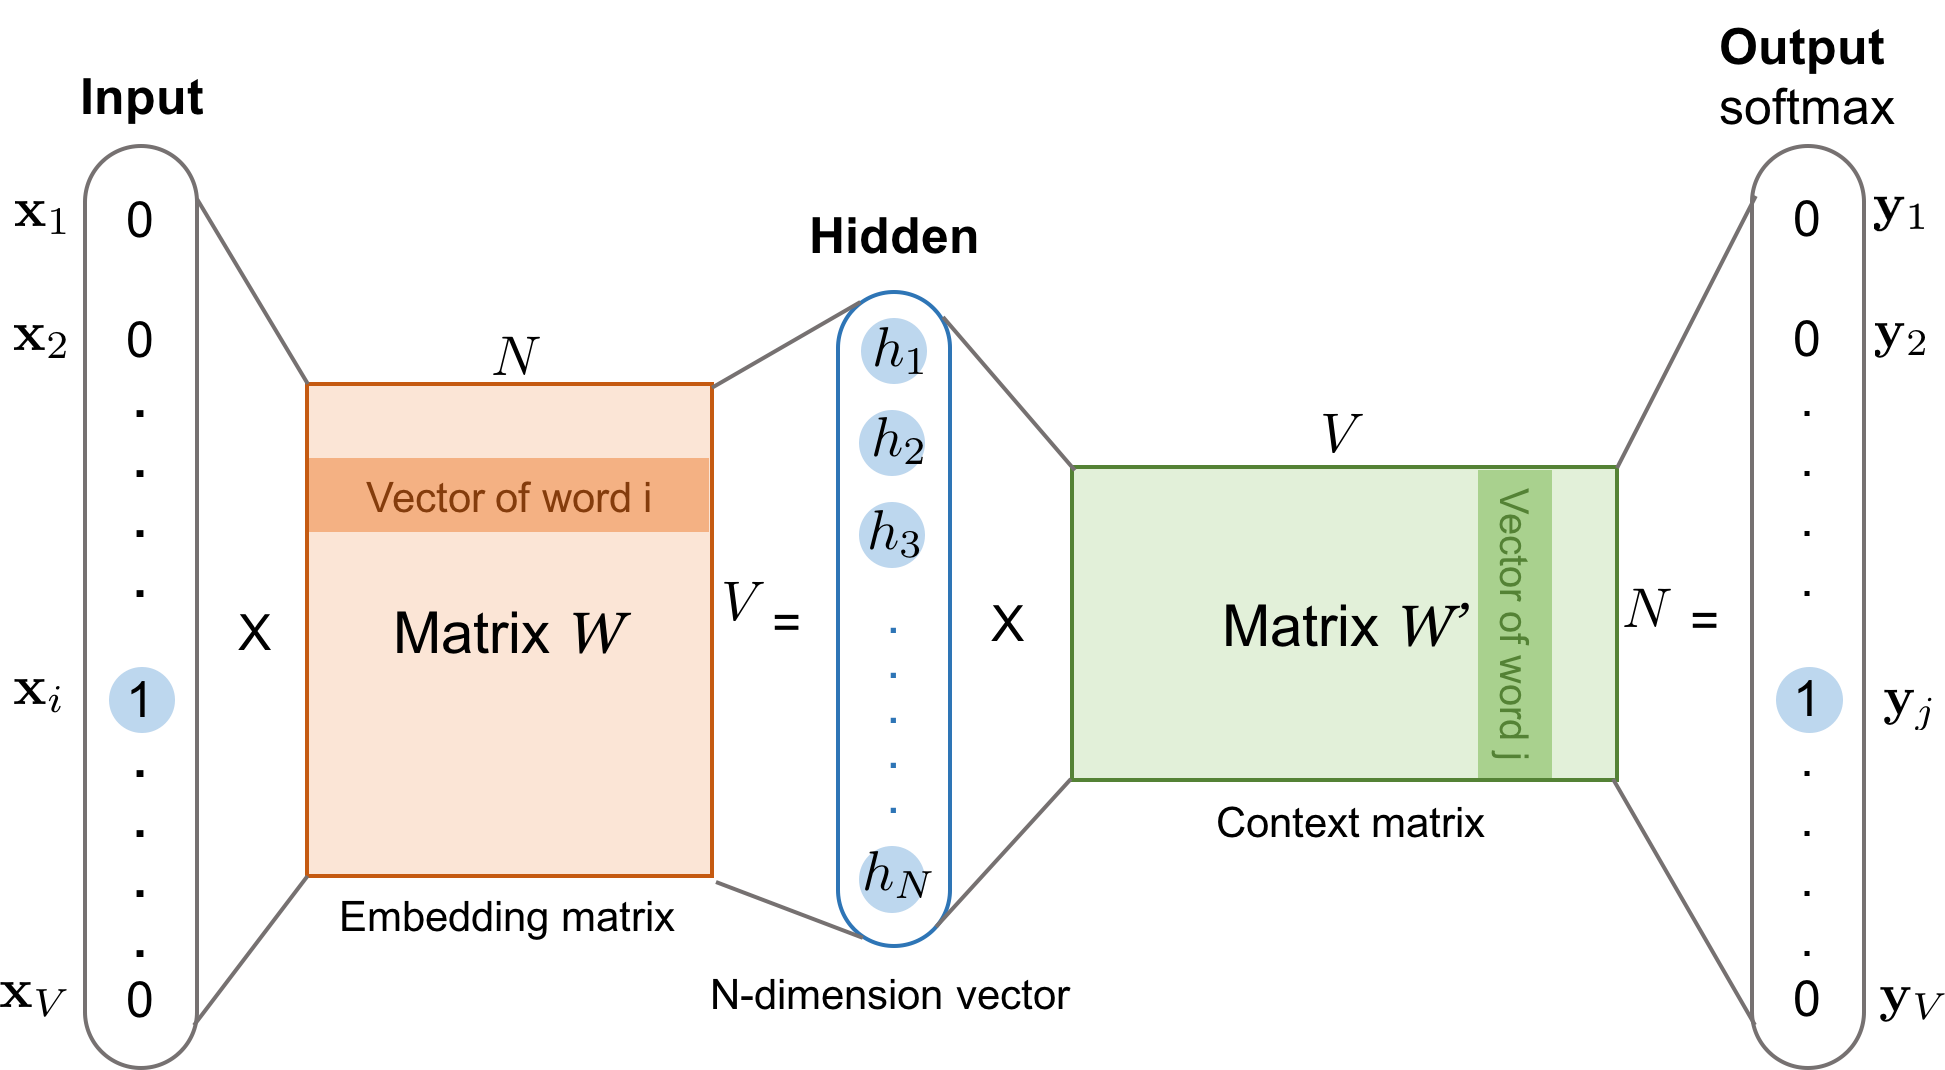
\includegraphics[scale = 0.3]{images/skip-gram.png}
\end{center}

\subsubsection{Word2Vec - Semantic and syntactic relations}
Word2vec captures different degrees of similarity between words. For example, patterns such as \textit{Man is to Woman as Brother is to Sister} can be generated through algebraic operations on the vectors representations of the words.
\[Brother - Man + Woman \approx Sister\]


\section{Syntactic Parsing}
Parsing is the process of analyzing a string of words to uncover its phrase structure, according
to the rules of a grammar.

\subsection{Dependency Parsing}
Which words depend on other words in our text data? What word is the “head” word in charge, so to speak? These are the questions answered by dependency parsing. This is the task of extracting a grammatical structure that clearly defines the relationships between “head” words and all other words. Thinking of it like a graph, the words are nodes and the dependencies between them are edges. Some specifically call this a Dependency Structure. In this structure, there is a defined root word. All other words can be reached (are dependent to) through this word as a starting point of the text data. 

\subsection{Constituency Parsing}
Where Dependency Parsing is based on dependency grammar, Constituency Parsing is based on context-free grammar. This type of parsing deals with the types of phrases in the text data. Constituency Parsing breaks text into sub-phrases, constituents, based on a grammar category. They are basically their own unit of grammar. Some categories for the phrase units of grammar are noun phrase (NP), verb phrase (VP) or sometimes prepositional phrase (PP).
